\documentclass[letterpaper, 12pt]{article}
\usepackage[margin=1in]{geometry}
\usepackage{amsmath}
\usepackage{amssymb}
\usepackage{fancyhdr}
%\usepackage{hyperref}
\usepackage{xcolor}
\usepackage{tikz}
\usepackage{pgfplots}
\usetikzlibrary{positioning, calc}
\setlength{\headheight}{15pt}

\pagestyle{fancy}
\fancyhf{}

\rhead{
    Shengdong Li
    Calc 1
}
\rfoot{
    Page \thepage
}

\usepackage{indentfirst}

\begin{document}
\title{Initial Post}
\author{by Shengdong Li}
\date{22 May 2020}
\maketitle

\section{Intro}
Hello everyone! For me, I chose to go into the Physics/Engineering lessons, so I'll try to give a summary of all the important topics covered, including finding the arc lengths of a curve, and using that arc length to find the surface area, then finding the center of mass of an object with different weighted densities.

\section{Arc Lengths}
Finding the arc length of a function is based off looking at the small rates of change and adding it up together, like most other formulas in calclulus. \par
First, imagine that a function is made up of a bunch of points connected together.
\begin{center}
    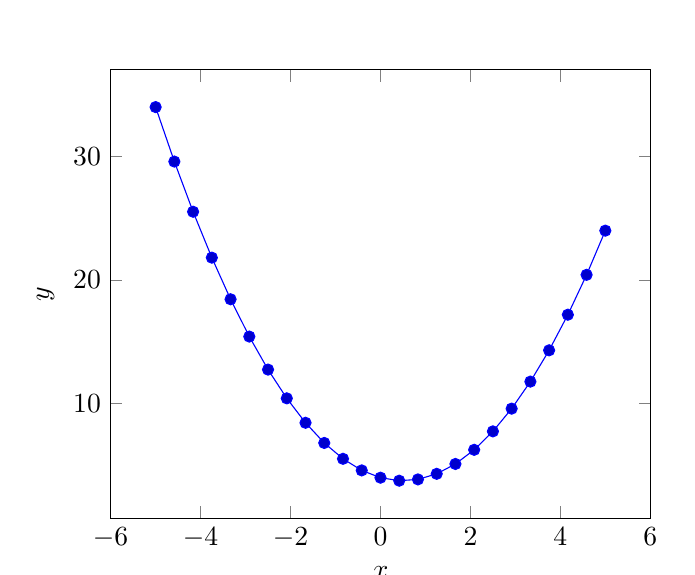
\begin{tikzpicture}
        \begin{axis}[
                xlabel=$x$,
                ylabel={$y$}
            ]
            % use TeX as calculator:
            \addplot {x^2 - x +4};
        \end{axis}
    \end{tikzpicture}
\end{center}
If you zoom in on one of these points, you'll find that you can calculate the length of this arc using the pythagorean theorem, imagining that the legs are $dx$ and $dy$.
\begin{center}
    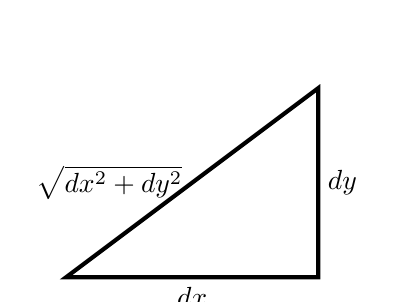
\begin{tikzpicture}[scale=0.8]
        % draw the background
        %\draw [line width=1.5pt, fill=gray!2] (0,0) -- (60:4) -- (4,0) -- cycle;

        \coordinate[label=left:$$]  (A) at (0,0);
        \coordinate[label=right:$$] (B) at (4,0);
        \coordinate[label=above:$$] (C) at (4,3);

        \coordinate[label=below:$dx$](c) at ($ (A)!.5!(B) $);
        \coordinate[label=left:$\sqrt{dx^2+dy^2}$](b) at ($ (A)!.5!(C) $);
        \coordinate[label=right:$dy$](a) at ($ (B)!.5!(C) $);

        %angle alpha
        %\draw[fill=red!30] (0,0) -- (0:0.75cm) arc (0:36.87:.75cm);
        %\draw (1cm,0.35cm) node {$\theta$};

        % angle beta
        %\begin{scope}[shift={(4cm,0cm)}]
        %    \draw[fill=green!30] (0,0) -- (-180:0.75cm) arc (180:120:0.75cm);
        %    \draw (150:0.5cm) node {$\beta$};
        %\end{scope}

        % angle gamma
        %\begin{scope}[shift={(60:4)}]
        %    \draw[fill=green!30] (0,0) -- (-120:.75cm) arc (-120:-60:.75cm);
        %    \draw (-90:0.5cm) node {$\gamma$};
        %\end{scope}

        % the triangle
        \draw [line width=1.5pt] (A) -- (B) -- (C) -- cycle;
    \end{tikzpicture}
\end{center}
Now we just have to find the infinite sum of all of the small lengths combined from a starting point to an end point, which would look a little something like $\int_{a}^{b}\sqrt{dx^{2}+dy^{2}}$. However, we can't have both $dx$ and $dy$ in one problem, so let's work on $dy$ and try to make it in terms of $dx$. \par
$dy$ can be rewritten as $f(b)-f(a)$. Now, to produce the $dx$, let's rewrite this expression with $dx$ divided and multiplied, which would look like this: $\frac{f\left(b\right)-f\left(a\right)}{dx}\cdot dx$ and $dx$ can be written as $b-a$. Doing that for the denominator of the fraction would result in $\frac{f\left(b\right)-f\left(a\right)}{b-a}\cdot dx$. The fraction on the left is the definition of a derivative, so this entire thing can then be rewritten as $f'\left(x\right)dx$. \par
Pluggin this into our total arc length would result in $\int_{a}^{b}\sqrt{dx^{2}+\left(f'\left(x\right)dx\right)^{2}}$. Now we can use some algebra to clean this up a bit.
\begin{align}
    \int_{a}^{b}\sqrt{dx^{2}+\left(f'\left(x\right)dx\right)^{2}} & =\int_{a}^{b}\sqrt{dx^{2}\left(1+f'\left(x\right)^{2}\right)} \\
                                                                  & =\boxed{\int_{a}^{b}\sqrt{1+f'\left(x\right)^{2}}dx}
\end{align}
Which is the final arc length formula.

\section{Centroids}
Honestly, centroids sound really complicated but become a lot easier once you start getting familiar with them by doing a few problems. \par
Centroids are the center of mass of some object. Unlike the geometric center of something, the center of mass factors in the mass of the function, at some specific point. As a result, the distance is weighted. \par
The final coordinate for the center of mass is something like this: $
    Center\ of\ Mass\left(COM\right)=\left(x_{COM},\ y_{COM}\right)=\boxed{\left(\frac{My}{m_{total}},\ \frac{Mx}{m_{total}}\right)}$ \par
\subsection{What is $My$ and $Mx$?}
$My$ is the \textbf{weighted distance} from the $y$-axis, and $Mx$ is the \textbf{weighted distance} from the $x$-axis. To find $My$, you multiply all the $x$ coordinates by the mass at that coordinate, and to find $Mx$, you multiply all the $y$ coordinates to find all the mass at that point. This explains why the final $COM$ actually has $Mx$ in the first place and $My$ following.
\subsection{What is $m_{total}$?}
$m_{total}$ is just the total mass at all points combined.
\subsection{Basic Example}
So say you're given two points,$\left(-1,-2\right)$, and $m$, the mass at that point, $=5$. Then $\left(1,2\right)$, and $m=3$ at that point, $m_{total}=5+3=8$. $My=\left(-1\right)\left(5\right)+\left(1\right)\left(3\right)=-2$, and $Mx=\left(-2\right)\left(5\right)+\left(2\right)\left(3\right)=-4$. The final $COM$ would be $
    \left(\frac{My}{m_{total}},\ \frac{Mx}{m_{total}}\right)$, which is actually $\left(\frac{-2}{8},\ \frac{-4}{8}\right)=\left(-\frac{1}{4},\ -\frac{1}{2}\right)$. If you now graph the points, you can clearly see that the $COM$ leans towards $\left(-1,-2\right)$, which had a greater mass.
\subsection{Applied to Calculus}
As you might expect, in calculus, instead of being given individual points, along with the mass, you might be given a mass function instead. \par
Say $p=density$, and $f(x)=mass\:function$, $M_{total}$ would be the area under the mass function,: $M=p\int_{a}^{b}f\left(x\right)dx$. Then $M_{x}$ would still be the $y$ coordinate multiplied by the mass at that point, which would be $M_{x}=p\int_{c}^{d}yf\left(y\right)dy$, and finally, $M_{y}=p\int_{b}^{a}xf\left(x\right)dx$.
\subsubsection{Some alternative formulas}
For when you don't want to put $Mx_{x}$ in terms of $y$, use $M_{x}=\frac{p}{2}\int_{a}^{b}f\left(x\right)^{2}dx$. \par
Then when working between curves, you can use something similar to the disk/washer method, where you subtract the top from the bottom function, like so $M_{x}=\frac{p}{2}\int_{a}^{b}y\left(f\left(y\right)-g\left(y\right)\right)dy$, and same principle for the $M_{y}$.
\section{History of the Arc Lengths}
One thing that I always find interesting about calculus formulas is how the formulas came to be. After doing some research online, it turns out that it took quite a while for the arc length formula to come about. \par
First, methods similar to Riemann Sums were used to find the area under a curve, brought forth by Archimedes. Various polygons were inscribed into the curve and the area under a curve, known as the method of exhaustion. Soon enough, this was also applied to the arc lengths, and the method of exhaustion could then be used to calculate arc lengths. The value of $\pi$ was approximated in this way.\par
As such, by using geometric methods, in the $17$th century, many proofs of the arc lengths of several functions came about. \par
Finally, \textit{Hendrik van Heurat} and \textit{Pierre de Fermat} independently came up with the form for the modern integral. Hendrik solved arc lengths by first finding the tangent line of a function at a certain point by finding the slope of the function at that point, and then incrementing a little bit to the right by some value. As you can see, this forms a bit of a triangle, in which he used the pythagorean theorem and got a formula similar to what we have today. He summed up a small number of these segments to approximate the arc length. \par
Learning about the history behind a formula makes me realize that it's ok that I don't understand the formula at first glance, and makes me motivated to keep learning it. 
\section{Conclusion}
I hope that my explanations for each topic were interesting and informative! Thanks for reading. \bigskip \par
Cheers, \par
Andy Li
\end{document}